Im Rahmen dieser Arbeit wird ein CRS entworfen und prototypisch implementiert, welches die besagten Kern-Anforderungen erfüllt. Die entstehende Software hört auf den Namen Weclare (ein Akronym für „\textbf{We}b \textbf{Cla}ssroom \textbf{Re}sponse (System)“. Der gesamte Quelltext zu dem Projekt findet sich in einem öffentlichen GitHub-Repository\cite{web:github_weclare} und eine öffentlich zugängliche Version der Software kann unter \texttt{www.weclare.de} aufgerufen werden. Insgesamt hat die entstandene Implementierung einen Umfang von rund 6000 Zeilen Code (vergleichbar mit dem Vorbild StuReSy).

Eine weitere Anforderung an das neue System: Zur Evaluierung soll Weclare auch mit bestehenden Datensätzen aus StuReSy funktionieren. Aus diesem Grund wird außerdem ein Kommandozeilen-Werkzeug entwickelt, welches Fragensätze vom XML-basierten StuReSy-Format in das JSON-basierte Weclare-Format konvertiert. Dieser Konverter wurde ebenfalls in JavaScript geschrieben und benötigt die Node.js-Laufzeitumgebung. Auch dieses Hilfsprogramm kann in einem öffentlichen GitHub-Repository\cite{web:github_converter} gefunden werden. 

\newpage
\section{Implementierung als Single Page Application mit dem React-Framework}
\label{chap:react_einfuehrung}
Um eine webbasierte Anwendung zu erstellen, die ohne einen zentralen Server auskommt, muss die Software komplett clientseitig in einem Browser ausgeführt werden, das heißt auch vollständig in JavaScript implementiert werden. Ein klassisches Backend, also eine Datenschicht (üblicherweise handelt es sich bei den meisten Web-Applikationen mindestens um eine Zwei-Schichten-Architektur) existiert nicht, beziehungsweise ist in die Präsentationsschicht integriert. Das bedingt die Kategorisierung einer solchen Anwendung als „Fat Client“.

Für diesen Zweck bietet es sich an, die Software als sogenannte „Single Page Application“ zu implementieren. Herkömmliche Webseiten, sogenannte Multi-Page-Applications werden während ihrer Lebenszeit mehrfach aktualisiert. Zum Beispiel jedes Mal, wenn der Server neues HTML liefert, das dargestellt werden soll. Eine Single Page Appliaction lädt nur eine einzige Webseite und das zugehörige JavaScript-Programm und verändert diese eine Seite dann im weiteren Verlauf dynamisch. Weitere Inhalte werden bei Bedarf asynchron (ohne Blockieren der Seite) nachgeladen, es wird jedoch keine neue Seite geladen. Damit wird auch eine hohe Autarkie gegenüber dem Webserver erreicht, da dieser nur mit wenigen Requests (im einfachsten Fall ein Request pro Nutzer) umgehen muss. Die Anforderungen an den Webserver auf dem die Anwendung bereitgestellt wird sind sehr gering, er muss lediglich statische Dateien (HTML, JavaScript, Bilder, Schriften, etc.) bereitstellen.

Als Framework für die Implementierung einer solchen Single Page Application wird das React-Framework\cite{web:react} ausgewählt. Das Open-Source-Projekt existiert seit 2013 und wird von Facebook finanziert. Es gehört zu den populärsten Frameworks zum Erstellen von Benutzeroberflächen und Web-Applikationen und ist dem Autor der Arbeit bereits vertraut.

Um einige Implementationsdetails nachzuvollziehen, erfolgt an dieser Stelle eine kleine Einführung in Grundkonzepte von React.

\subsection{Komponenten und State}
Die elementaren Bausteine einer React-Anwendung sind \texttt{Komponenten}. Die React-Dokumentation beschreibt die Aufgabe von Komponenten wie folgt\cite{web:react}:
\begin{quotation}
„Build encapsulated components that manage their own state, then compose them to make complex UIs.“
\end{quotation}

Ein Komponente ist eine autarke und wiederverwendbare Einheit und kapselt meistens sowohl Struktur, Aussehen als auch Logik. Komponenten werden häufig als Klasse implementiert (können aber in einfachen Fällen auch als Funktion implementiert werden) und erben von der Klasse \texttt{React.Component}. Valide Komponenten müssen über eine \texttt{render()}-Funktion verfügen, die HTML oder andere React-Komponenten zurückliefert. Eine sehr simple, statische Komponente könnte so aussehen:

\begin{minipage}{\linewidth}
\begin{lstlisting}[caption={Einfache React-Komponente ohne JSX-Syntax.}]
import React from "react";

class Greeting extends React.Component {
  render() {
    return React.createElement("div", null, "Hello there!");
  }
}
\end{lstlisting}
\end{minipage}

Da der Aufruf \texttt{React.createElement()} nicht so schön zu lesen ist, wie die Notation eines XML-Tags (\texttt{<div>...</div>}) wird im React-Umfeld häufig eine Syntax-Erweiterung namens JSX (JavaScript Syntax Extension) verwendet um React-Komponenten zu beschreiben. JSX wird mit einem Compiler während des Build-Prozesses in herkömmliches JavaScript umgewandelt. Äquivalent zum letzten Beispiel wäre daher die folgende Variante unter Einbeziehung von JSX-Syntax:

\begin{minipage}{\linewidth}
\begin{lstlisting}[caption={Einfache React-Komponente mit JSX-Syntax.}]
import React from 'react';

class Greeting extends React.Component {
    render() {
        return <div>Hello there!</div>;
    }
}
\end{lstlisting}
\end{minipage}

Um Komponenten dynamisch zu machen, können über sogenannte \texttt{Properties} Daten an Komponenten übergeben werden:

\begin{minipage}{\linewidth}
\begin{lstlisting}[caption={Komponenten erhalten Daten über ihre Properties.}]
import React from "react";

class Greeting extends React.Component {
  render() {
    return <div>Hello, {this.props.name}!</div>;
  }
}
\end{lstlisting}
\end{minipage}

Properties werden wie andere HTML-Attribute auch einfach hinter den Namen der Komponente innerhalb des zugehörigen Tags in die Instanziierung einer Komponente integriert:

\begin{minipage}{\linewidth}
\begin{lstlisting}[caption={Properties werden wie normale HTML-Attribute verwendet.}]
import React from "react";

class GreetAllFriends extends React.Component {
  render() {
    return (
      <div>
        <Greeting name="Michael" />
        <Greeting name="Karla" />
      </div>
    );
  }
}
\end{lstlisting}
\end{minipage}

\texttt{Properties} werden also verwendet um Daten in Komponenten hinein zu reichen. React kümmert sich automatisch um das Aktualisieren der aktuellen Ansicht, sobald sich eine Property ändert (dieses „reaktive“ Prinzip ist auch der Namensgeber für das Framework). Dabei verwendet React sehr schnelle und intelligente Algorithmen, um immer nur diejenigen Elemente einer Seite zu aktualisieren, die sich auch tatsächlich geändert haben.

Properties können nicht modifiziert werden – sie sind wie auch die meisten anderen Objekte innerhalb von React „immutable“. Wenn Daten innerhalb einer Komponente modifiziert werden sollen, gehören sie in das interne, modifizierbare \texttt{state}-Objekt dieser Komponente:

\begin{minipage}{\linewidth}
\begin{lstlisting}[caption={Jede Komponente kann über einen modifizierbaren state verfügen.}]
import React from "react";

class BusyOrNot extends React.Component {
  state = {
    busy: false
  };

  toggleBusy() {
    this.setState(prevState => ({
      busy: !prevState.busy
    }));
  }

  render() {
    return (
      <div>
        <div>This user is {busy ? "busy" : "not busy"}!</div>
        <button type="button" onClick={this.toggleBusy}>
          Change Busy State
        </button>
      </div>
    );
  }
}
\end{lstlisting}
\end{minipage}

Bedingt durch die statische Natur der Properties, forciert React einen unidirektionalen Datenfluss. Daten können nur von „oben nach unten“ (in Bezug auf die Baumstruktur im Document Object Model einer Seite) durch eine Anwendung fließen. Möchten zwei Komponenten an unterschiedlichen Stellen auf die gleichen Daten zugreifen, dann sollten diese in einer gemeinsamen Eltern-Komponente gehalten werden. \newline

\begin{minipage}{\linewidth}
\begin{lstlisting}[caption={„Lifting state up“: Mehrere Komponenten greifen auf die gleichen Daten zu.}]
import React from "react";

function Son(props) {
  return <p>I am the son of {props.parent}</p>
}

function Daughter(props) {
  return <p>I am the daughter of {props.parent}</p>
}

class Parent extends React.Component {
  state = {
    parentName: "Peter Parent"
  };

  render() {
    return (
      <div>
        <Son parent={this.state.parentName} />
        <Daughter parent={this.state.parentName} />
      </div>
    );
  }
}
\end{lstlisting}
\end{minipage}

Da dieses Muster bei großen Anwendungen aber schnell zu sehr aufwendigem „Durchstecken“ von Properties (Prop Drilling) durch mehrere Komponenten-Ebenen führt, gibt es eine populäre Erweiterung für React zur Verwaltung eines globalen States in der gesamten Anwendung: das Flux-Muster.


\subsection{State Management mit Redux}
Das Flux-Entwurfsmuster ist ebenfalls eine Entwicklung von Facebook. Prinzipiell handelt es sich um ein abstraktes Entwurfsmuster, das in vielen Sprachen angewendet werden kann. Etabliert hat es sich jedoch gerade in Kombination mit React-Anwendungen. Die bekannteste Implementation, die auch in dieser Arbeit verwendet wird, hört auf den Namen Redux \cite{web:redux}.

Im Flux-Muster geht es darum, eine zentrale Zustandsverwaltung für eine Anwendung einzurichten, eine sogenannte „Single Source of Truth“. Dieser zentrale Ort wird als „Store“ bezeichnet. Ein Store beinhaltet typischerweise solche Daten, die für die gesamte Anwendung relevant sind. Parallel dazu kann es aber weiterhin Komponenten geben, die einen eigenen, lokalen State verwalten, wenn dieser nicht für die gesamte Anwendung relevant ist (zum Beispiel der Status von einzelnen UI-Elementen).

\begin{figure}[H]
    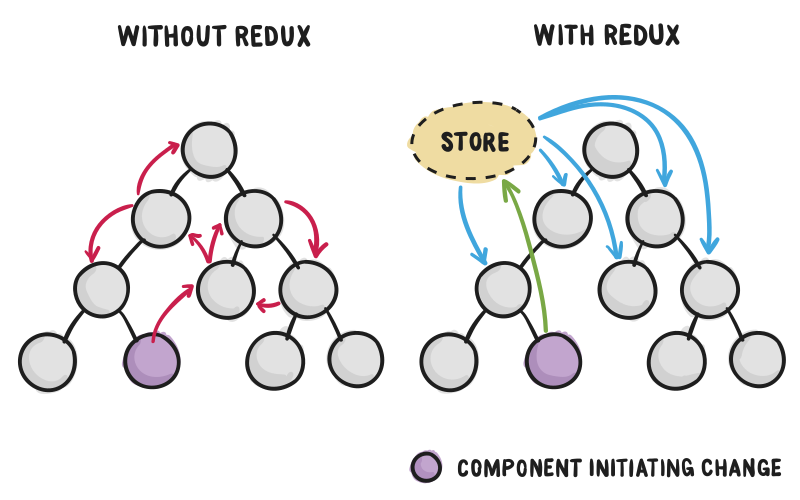
\includegraphics[width=12cm]{chapter/entwurf/BA_redux.png}
    \centering
    \caption{Der Redux-Store verwaltet den globalen Zustand einer React-Anwendung und ist die „Single Source of Truth“. Quelle: https://css-tricks.com/learning-react-redux/ (aufgerufen am 24.4.19)}
    \label{Abbildung 4.1.3}
\end{figure}


Einzelne React-Komponenten können mit einem Store durch einen Publish/Subscribe-Mechanismus verbunden werden. Die gewünschten Daten aus dem Store stehen der Komponente dann als Properties zur Verfügung. Ändern sich die Daten im Store, dann wird die verbundene Komponente sofort benachrichtigt und bei einer Änderung der Properties auch neu gerendert (reaktives Prinzip). Um eine möglichst lose Kopplung zwischen den Komponenten zu realisieren, wird empfohlen die Verbindung zu einem Store in einer (nicht sichtbaren) Container-Komponente zu realisieren. In diesem Beispiel wird die eigentliche, sichtbare \texttt{Header}-Komponente mit einem unsichtbaren Container versehen, der die notwendigen Daten aus dem Store innerhalb der Komponente unter der \texttt{status}-Property verfügbar macht.

\begin{minipage}{\linewidth}
\begin{lstlisting}[caption={Über den connect-Aufruf beim Exportieren der Komponente wird sie mit dem Store verbunden.}]
import { connect } from "react-redux";
import Header from "./Header";

const mapStateToProps = state => ({
  status: state.connection.status
});

export default connect(mapStateToProps)(Header);
\end{lstlisting}
\end{minipage}

Ähnlich wie die Properties in React, sind auch die Daten in einem Store unveränderlich. Änderungen in einem Store müssen mithilfe von \texttt{Actions} realisiert werden. Bei einer Action handelt es sich lediglich um ein Objekt, welches die Art der Änderung in einem Store beschreibt. Um das wiederholte Schreiben aufwändiger Objekt-Literale zu erleichtern werden die Actions üblicherweise von einer \texttt{ActionCreator}-Funktion erzeugt:

\begin{minipage}{\linewidth}
\begin{lstlisting}[caption={Ein Action-Objekt ist lediglich die Beschreibung einer Änderungsoperation und wird in einem ActionCreator erzeugt.}]
export function addQuestion(newQuestion) {
  return {
    type: "ADD_QUESTION",
    payload: {
      newQuestion
    }
  };
}
\end{lstlisting}
\end{minipage}

Die Implementierung einer Änderungsoperation erfolgt in dem zugehörigen \texttt{reducer}. Die Operationen in einem reducer sind stets pure Funktionen, das heißt sie liefern immer das gleiche Ergebnis bei gleichen Eingabe-Parametern und sie haben keine Seiteneffekte. Die Parameter des reducers sind immer der aktuelle State und die eingehende Action. Ein einfacher Reducer zum Hinzufügen einer Frage zu einem Fragekatalog könnte so aussehen:

\begin{minipage}{\linewidth}
\begin{lstlisting}[caption={In einem Reducer werden die Änderungsoperationen eines Stores als pure Funktion implementiert.}]
const questionEditor = (state = [], action) => {
  switch (action.type) {
    case "ADD_QUESTION": {
      return [... state, createNewQuestion()];
    }
  }
};
\end{lstlisting}
\end{minipage}

\subsection{Konkrete Umsetzung am Beispiel des Fragen-Editors}
Um das neue CRS zu implementieren, muss zuerst eine sinnvolle Aufteilung in Komponenten erfolgen. Exemplarisch soll an dieser Stelle einer der Hauptbestandteile der Anwendung besprochen werden: der Fragen-Editor.

Das zweiteilige Design, bestehend aus einer Fragenliste in der Seitenspalte und einem Fragen-Inhaltsbereich, das sowohl bei StuReSy als auch bei Pingo zum Einsatz kommt, soll beibehalten werden.

Eine mögliche Komponenten-Hierarchie für den Fragen-Editor wird in \ref{Abbildung 4.1} veranschaulicht. Die äußerste Komponente, der \texttt{QuestionEditorContainer} ist nicht sichtbar, es handelt sich dabei um eine Container-Komponente, welche die notwendigen Daten aus dem Store holt und dann an seine Kinder-Komponenten mittels Properties weitergibt.

\begin{figure}[H]
    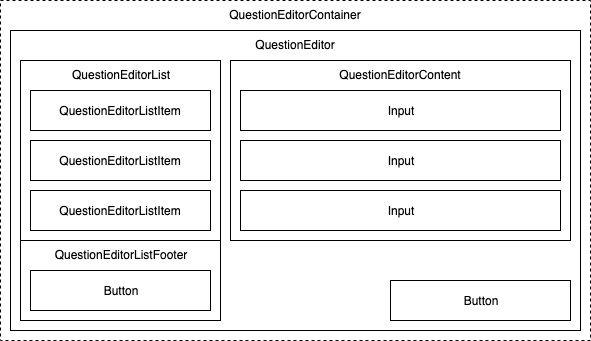
\includegraphics[width=12cm]{chapter/entwurf/Component_Hierarchy.png}
    \centering
    \caption{Mögliche Komponenten-Hierarchie für den Fragen-Editor.}
    \label{Abbildung 4.1}
\end{figure}

Die tatsächliche Implementierung entspricht nahezu vollständig diesem Bild (einzig die Komponente \texttt{QuestionEditorListItem} findet sich nicht im fertigen Ergebnis.

\begin{figure}[H]
    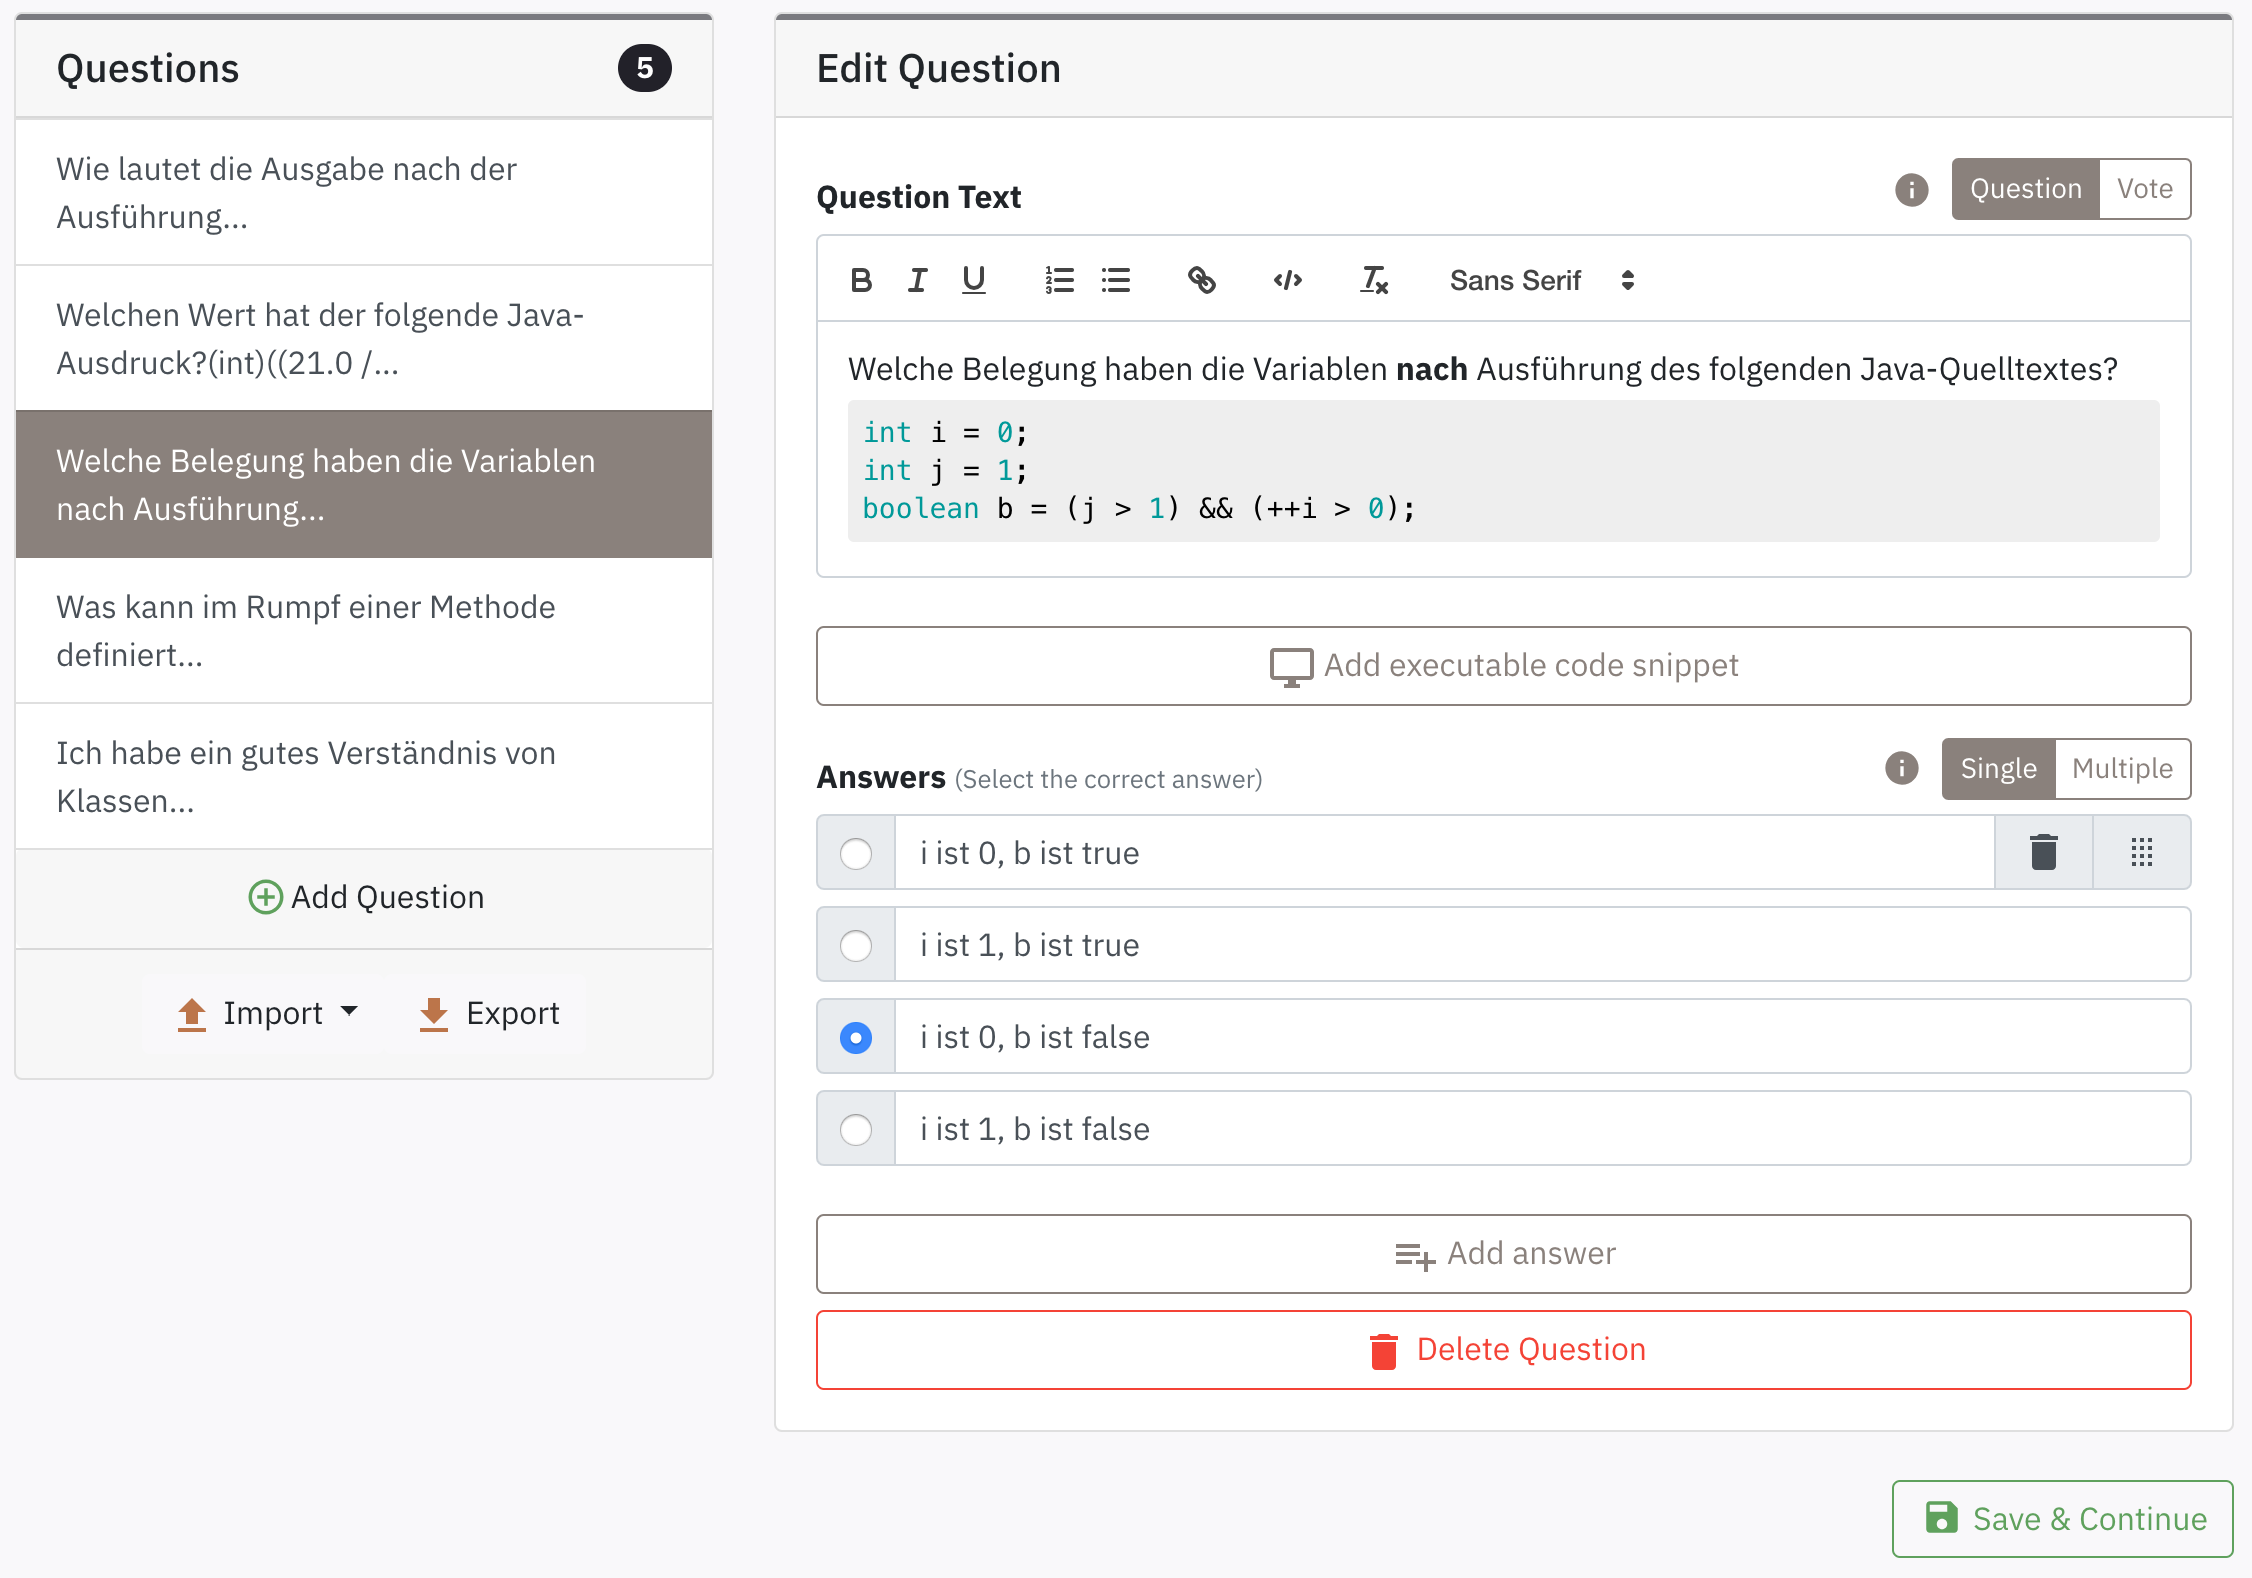
\includegraphics[width=16cm]{chapter/entwurf/weclare_editor.png}
    \centering
    \caption{Fertige Implementierung des Fragen-Editors im React-Framework.}
    \label{Abbildung 4.2}
\end{figure}

Alle Daten des Fragen-Editors werden in einem einzigen Redux-Store gehalten. Alle möglichen Änderungen finden sich in einem zugehörigen Reducer wieder, der auszugsweise wie folgt aussieht:


\begin{minipage}{\linewidth}
\begin{lstlisting}[caption={Auszug aus dem Reducer für den Fragen-Editor.}]
export const questionEditor = (state = [], action) => {
  switch (action.type) {
    case ADD_QUESTION: {...}
    case EDIT_QUESTION_TEXT: {...}
    case EDIT_QUESTION_CODE: {...}
    case EDIT_QUESTION_MODE: {...}
    case EDIT_QUESTION_TYPE: {...}
    case DELETE_QUESTION: {...}
    case DELETE_ANSWER: {...}
    case ADD_ANSWER: {...}
    case EDIT_ANSWER_TEXT: {...}
    case SET_CORRECT_SINGLE_ANSWER: {...}
    case SET_CORRECT_MULTI_ANSWER: {...}
    case LOAD_QUESTIONS: {...}
    case SORT_QUESTION: {...}
    case SORT_ANSWER: {...}
    default: {
      return state;
    }
  }
};
\end{lstlisting}
\end{minipage}


\newpage
\section{P2P-WebRTC-Verbindungen mit PeerJS}
\label{chap:p2p}
Um Unabhängigkeit von einem dedizierten, zentralen Anwendungsserver zu erlangen, der einerseits Wartungsaufwand bedeutet, und außerdem einen „Single Point of Failure“ darstellt, werden Verbindungen direkt zwischen den Teilnehmern aufgebaut. Jeder Weclare-Nutzer kann zum Start einer Sitzung, also zur Laufzeit, entscheiden, welche Rolle er in der aktuellen Sitzung einnehmen will (Server oder Client). Der Rechner des Dozenten agiert typischerweise als Server, die Rechner der Studenten sind Clients und somit ergibt sich eine klassische, zentralisierte Architektur des verteilten Systems in Form einer Stern-Topologie. Unabhängig von der Wahl wird jedoch stets der gleiche Code vom Server geladen. Das Programm ist in dieser Hinsicht also omnipotent.

\begin{figure}[H]
    \centering
    \setlength{\fboxsep}{0pt}
    \setlength{\fboxrule}{0.5pt}
    \fbox{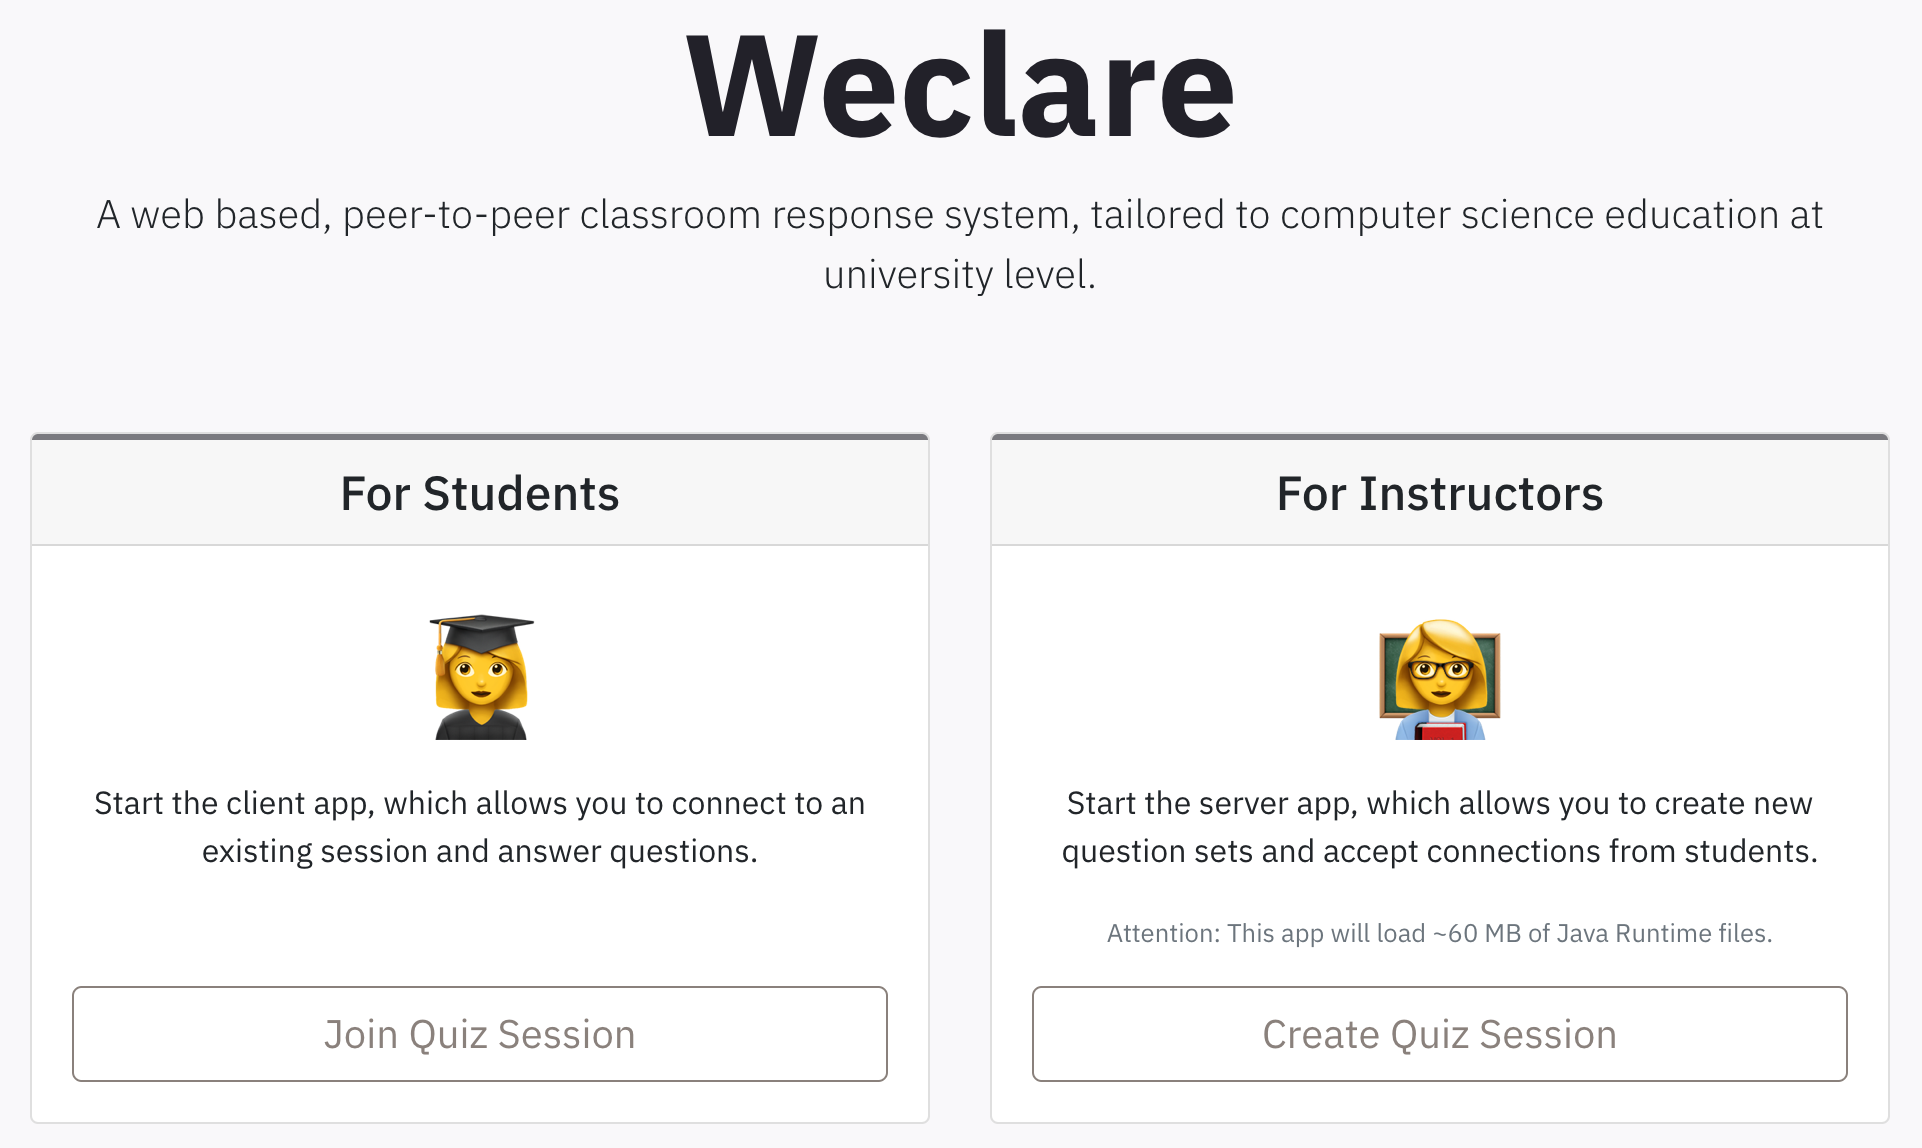
\includegraphics[width=\textwidth-1pt]{chapter/entwurf/bilder/weclare_start.png}}
    \caption[Start einer neuen Weclare-Sitzung]{Am Start einer Sitzung kann der Nutzer entscheiden, ob er als Client oder als Server teilnehmen möchte. Unabhängig von der Wahl wird das gleiche Programm geladen.}
    \label{abb:weclare_start}
\end{figure}

Mit diesem Verhalten erfüllt die Software die Definition einer Peer-to-Peer Architektur, zum Beispiel gemäß Tanenbaum\cite[S. 62]{book:tanenbaum}:

\begin{quotation}
„Aus einem übergeordneten Blickwinkel heraus sind die Prozesse, die ein Peer-to-Peer-System bilden, alle gleich. Die Funktionen, die ausgeführt werden müssen, werden also von jedem Prozess des verteilten Systems dargestellt. Folglich ist die meiste Interaktion zwischen Prozessen symmetrisch: Jeder Prozess agiert gleichzeitig als Client und als Server [...].“
\end{quotation}

Jedoch trifft dies nur auf den Zeitraum vor dem Start einer Sitzung zu. Sobald eine Sitzung begonnen hat, handelt es sich um eine klassische Client-Server-Struktur. Die Bezeichnung als Peer-to-Peer-Architektur entspricht daher nicht der gängigen Vorstellung eines vollvermaschten Peer-to-Peer-Netzwerks, bei dem jeder Teilnehmer mit jedem anderen Teilnehmer verbunden ist.

Die Tatsache, dass jeder Teilnehmer entscheiden kann, ob er als Server oder Client teilnehmen will, bedeutet auch, dass Aspekte wie Network Address Translation (NAT) und Firewalls beim Austausch der IP-Adressen (Signaling) berücksichtigt werden müssen.

Der Zugriff auf die Schnittstellen des Betriebssystems (wie etwa das Netzwerk) durch Browser-Skripte ist aus Sicherheitsgründen stark eingeschränkt. Viele bestehende webbasierte CRS (zum Beispiel Pingo, vgl. \cite{web:pingo_github}) verwenden das WebSocket-Protokoll zur Kommunikation zwischen Client und Server. Der WebSocket-Standard beschreibt jedoch nur Möglichkeiten zum Verbinden mit einem bestehenden Server aus dem Browser heraus, nicht zum Kreieren einer Verbindung (vgl. \cite{std:websockets}). Eine Peer-to-Peer-Architektur mit WebSockets ist deswegen nicht realisierbar.

Die einzige Möglichkeit, eine omnidirektionale Verbindung zwischen zwei Browsern zu realisieren, ist der relativ neue und offene WebRTC-Standard (Web Real-Time Communication)\footnote{Offizielle Webseite: \url{https://webrtc.org/}}. WebRTC wird hauptsächlich für Multimedia-Echtzeit-Anwendungen eingesetzt und seit 2017 von allen großen Browsern (Google Chrome, Mozilla Firefox, Opera, Apple Safari und Microsoft Edge) unterstützt. Viele Video- und Audiotelefonie-Lösungen (zum Beispiel Skype oder Discord) basieren inzwischen auf dem WebRTC-Protokoll. Neben Audio- und Videoinhalten können aber auch beliebige andere Daten über sogenannte \texttt{RTCDataChannel} übertragen werden. WebRTC beinhaltet keine Anweisungen für den Austausch der IP-Adressen zwischen beteiligten Parteien. Dieser Teil, das sogenannte Signaling, ist nicht Teil des Standards und muss selbst implementiert werden (vgl. \cite{web:webrtc_signaling}).

Der Aufwand dafür ist groß, weil viele verschiedene Netzwerk-Situationen berücksichtigt werden müssen. Deswegen wird beim Weclare-Prototypen eine OpenSource-Bibliothek namens PeerJS\footnote{Offizielle Webseite: \url{https://peerjs.com/}} verwendet, die WebRTC in eine sehr einfache API kapselt und ein Signaling-Verfahren beisteuert.

Die (in Kapitel \ref{chap:anforderung_p2p}) formulierte Anforderung, keinen dedizierten Server zu benötigen, kann aufgrund des notwendigen Signalings also nicht vollständig erfüllt werden und muss präzisiert werden: Ein Server wird lediglich zum Austausch der IP-Adressen der Teilnehmer benötigt. Nach dem Austausch ist kein Server mehr notwendig. Anwendungsdaten werden nie über einen zentralen Server, sondern immer nur zwischen den einzelnen Teilnehmern verschickt. Der notwendige Signaling-Server muss nicht vom Weclare-Anwender betrieben werden – ein öffentlicher Server kann verwendet werden. In der Standard-Einstellung verwendet PeerJS einen kostenlosen und öffentlichen Signaling-Server, der von den PeerJS-Autoren betrieben wird.

Die PeerJS-Library ermöglicht den Aufbau einer Datenverbindung zwischen zwei Browsern mit sehr simplen Aufrufen: Zunächst müssen Client und Server ein Peer-Objekt erzeugen. Als Parameter kann an dieser Stelle eine (auf dem Signaling-Server noch nicht verwendete) alphanumerische ID übergeben werden, unter welcher der zugehörige Peer beim Signaling-Server bekannt gemacht wird. Optional kann hier außerdem ein eigener Signaling-Server angegeben werden. 

Anschließend können an dem neuen Peer-Objekt diverse Callback-Methoden registriert werden, die den weiteren Gebrauch regeln. So kann zum Beispiel der Server seine neu erstellte ID kundtun und auf eingehende Verbindungen und Daten reagieren:

\begin{minipage}{\linewidth}
\begin{lstlisting}[caption={Verbindungsaufbau mit der PeerJS-Bibliothek auf der Server-Seite. (aus: src/server/actions/server.js)}]
import Peer from "peerjs";

const peer = new Peer("server-id");

peer.on("open", id => {
  console.log(`Successfully created peer: ${id}`);
});

peer.on("connection", conn => {
  console.log(`New client connected: ${conn.peer}`);
  conn.on("data", data => {
    switch (data.type) {
      case "answer":
        // Do something
        break;
      default:
      // Noop
    }
  });
});
\end{lstlisting}
\end{minipage}

Auf der Gegenseite, beim Client kann die Verbindung einfach über die \texttt{connect()}-Methode aufgebaut werden, die als Parameter die ID des gewünschten Peers erhält. Anschließend kann über das zurückgelieferte \texttt{Connection}-Objekt eine Nachricht verschickt werden. (vgl. \cite{web:peerj_docs})

\begin{minipage}{\linewidth}
\begin{lstlisting}[caption={Verbindungsaufbau mit der PeerJS-Bibliothek auf der Client-Seite. (aus: src/client/actions/client.js)}]
import Peer from "peerjs";

const peer = new Peer();
const connection = peer.connect("server-id");
connection.send("Hello world!");
\end{lstlisting}
\end{minipage}

Um dem Flux-Muster (siehe Kapitel \ref{chap:redux_state_management}) treu zu bleiben, wird die gesamte Netzwerk-Kommunikation innerhalb von ActionCreator-Funktionen implementiert. Da Netzwerk-Aufrufe keine puren Funktionen sind und asynchron erfolgen müssen, können sie nicht in einen Reducer integriert werden. Um solche asynchronen Actions zu realisieren, wird Redux um eine sehr simple Middleware namens \texttt{redux-thunk}\footnote{Offizielle Webseite: \url{https://github.com/reduxjs/redux-thunk}} erweitert. Diese Middleware erlaubt es, asynchrone Aufrufe in ActionCreator-Methoden unterzubringen (vgl. \cite{web:redux_async_actions}). Da viele dieser Netzwerkaufrufe eigentlich keine Änderungen im Store bewirken, wird der ActionCreator seinem Namen nicht mehr treu, denn am Ende wird, entgegen seinem Zweck, keine Action mehr zurückgegeben.

\begin{minipage}{\linewidth}
\begin{lstlisting}[caption={ActionCreator zum Versenden von Antworten vom Client zum Server. (aus: src/client/actions/client.js)}]
export function sendAnswers(answerIdxArray) {
  return (dispatch, getState) => {
    const {
      client: { connection = null, currentQuestion = null }
    } = getState();

    if (
      connection &&
      currentQuestion &&
      typeof answerIdxArray !== "undefined"
    ) {
      const msg = {
        type: "answer",
        payload: {
          questionIdx: currentQuestion.questionIdx,
          answerIdxArray,
          userId: connection.provider.id
        }
      };
      connection.send(msg);
    }
  };
}
\end{lstlisting}
\end{minipage}


\newpage
\section{Text- und Code-Formatierung mit Quill und CodeMirror}
\label{chap:formatierung}
Quelltexte können in zwei verschiedenen Kontexten in Fragestellungen auftauchen: Einerseits gibt es unvollständige, kurze Quelltext-Fragmente, die in einen Fließtext eingebunden werden sollen, wie in diesem Beispiel:

\begin{quote}
„Wie viele String-Parameter hat die folgende Java-Methode?\newline
public String m(int i, int s, boolean b) \{ ... \}“
\end{quote}

Dabei handelt es sich nicht um ein syntaktisch nicht vollständiges und nicht-ausführbares Java-Fragment. Um die Lesbarkeit dieses Fragments zu erhöhen, sollte es dennoch optisch deutlich vom Fließtext unterscheidbar sein. Es bietet sich an, den Code in einer Monospace-Schriftart zu formatieren und (wenn möglich) eine syntaktische Einfärbung (Syntax Highlighting) anzuwenden.

Da die Entwicklung einer eigenen Editor-Komponente komplex ist, und es in diesem Bereich bereits eine große Auswahl an Bibliotheken gibt, wird auf eine bestehende Implementierung zurückgegriffen. Dabei müssen folgende Anforderungen von einer solchen Bibliothek erfüllt werden:

\begin{itemize}
    \item \textbf{Integration in React:}  Muss sich leicht in das deklarative React-Framework einbinden lassen.
    \item \textbf{WYSIWYG (What You See Is What You Get):} Der Editor muss stets eine Vorschau aller Formatierungen darstellen, und es soll nicht zwischen einem Markup- und einem Vorschau-Modus gewechselt werden müssen. Formatierungen sollen über Buttons eingefügt werden können.
    \item \textbf{Text-Formatierungen:} Der Editor muss über simple Text-Formatierungen verfügen (zum Beispiel Fettschrift und Kursivierung).
    \item \textbf{Monospace-Schriftart:} Eine Möglichkeit zum Verwenden einer Monospace-Schriftart muss vorhanden sein.
    \item \textbf{Syntax-Highlighting:} Syntaktische, farbliche Hervorhebungen von Code-Fragmenten müssen unterstützt werden (üblicherweise durch ein Plugin/Erweiterung mit einer zusätzlichen Bibliothek wie Highlight.js).
\end{itemize}

Nach dem Erwägen und Ausprobieren diverser Bibliotheken (zum Beispiel Draft.js, Slate, Prosemirror, Quill) fiel die Wahl letztendlich auf den Quill-Editor\footnote{Offizielle Webseite: \url{https://quilljs.com/}}, der alle genannten Anforderungen erfüllt. Quill ist nicht primär für den Einsatz mit React vorgesehen, deswegen wird der Editor in Form der Wrapper-Bibliothek \texttt{react-quill}-Bibliothek\footnote{Offizielle Webseite: \url{https://github.com/zenoamaro/react-quill}} verwendet, die Quill in React-Komponenten bündelt.

\begin{figure}[H]
    \centering
    \setlength{\fboxsep}{0pt}
    \setlength{\fboxrule}{0.5pt}
    \fbox{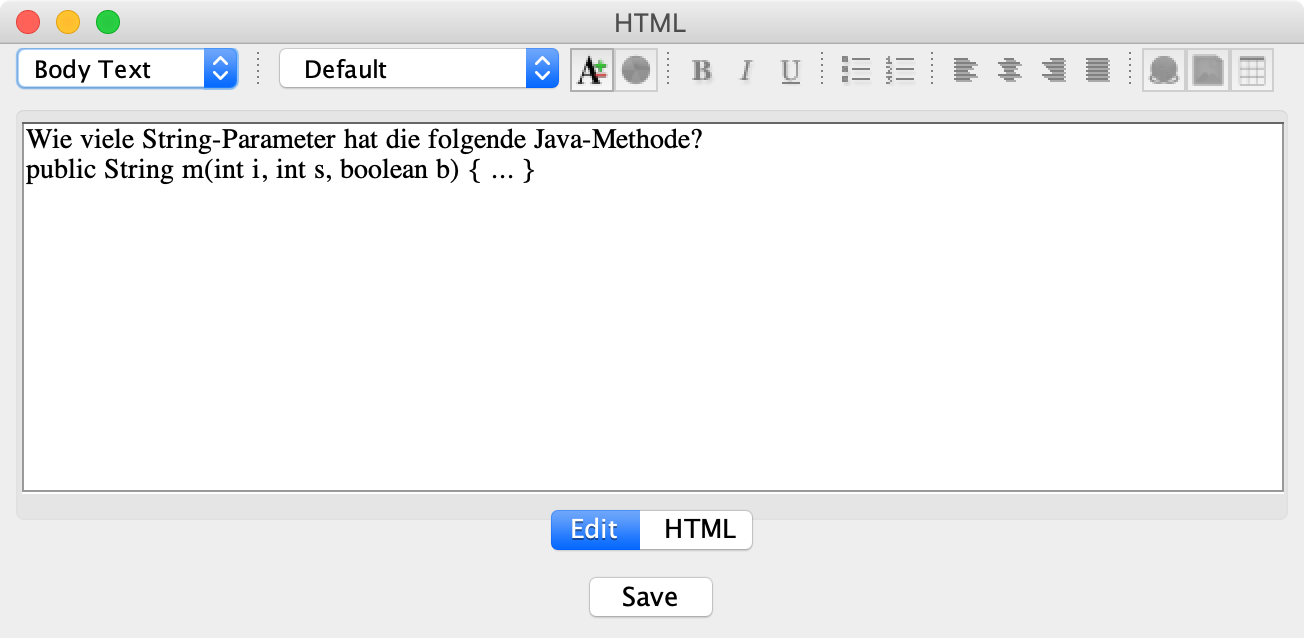
\includegraphics[width=\textwidth-1pt]{chapter/entwurf/bilder/sturesy_editor.png}}
    \caption[StuReSy-Fragen-Editor]{Bearbeiten einer Fragestellung im StuReSy-Fragen-Editor.}
    \label{abb:sturesy_editor}
\end{figure}

\begin{figure}[H]
    \centering
    \setlength{\fboxsep}{0pt}
    \setlength{\fboxrule}{0.5pt}
    \fbox{
\includegraphics[width=\textwidth-1pt]{chapter/entwurf/bilder/sturesy_fragment.png}}
    \caption[Darstellung eines Code-Fragments in StuReSy]{Darstellung eines Code-Fragments in StuReSy (ohne manuell vorgenommene Formatierungen)}
    \label{abb:sturesy_code_fragment}
\end{figure}


\begin{figure}[H]
    \centering
    \setlength{\fboxsep}{0pt}
    \setlength{\fboxrule}{0.5pt}
    \fbox{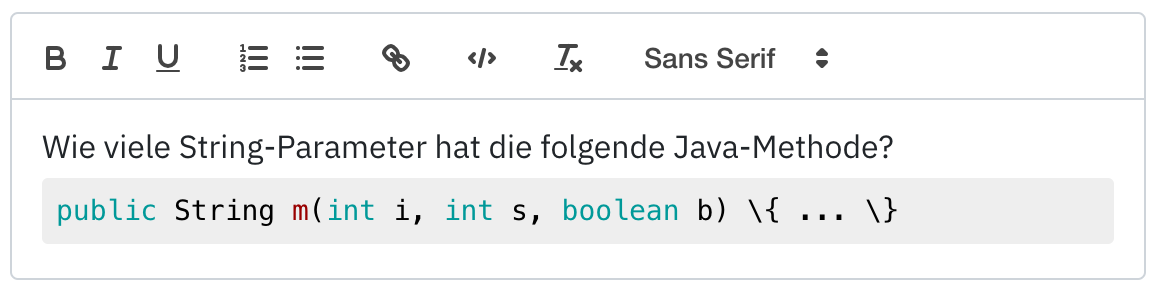
\includegraphics[width=\textwidth-1pt]{chapter/entwurf/bilder/weclare_quill.png}}
    \caption[Quill-Editor von Weclare]{Bearbeiten einer Fragestellung im Quill-Editor von Weclare.}
    \label{abb:weclare_quill}
\end{figure}

\begin{figure}[H]
    \centering
    \setlength{\fboxsep}{0pt}
    \setlength{\fboxrule}{0.5pt}
    \fbox{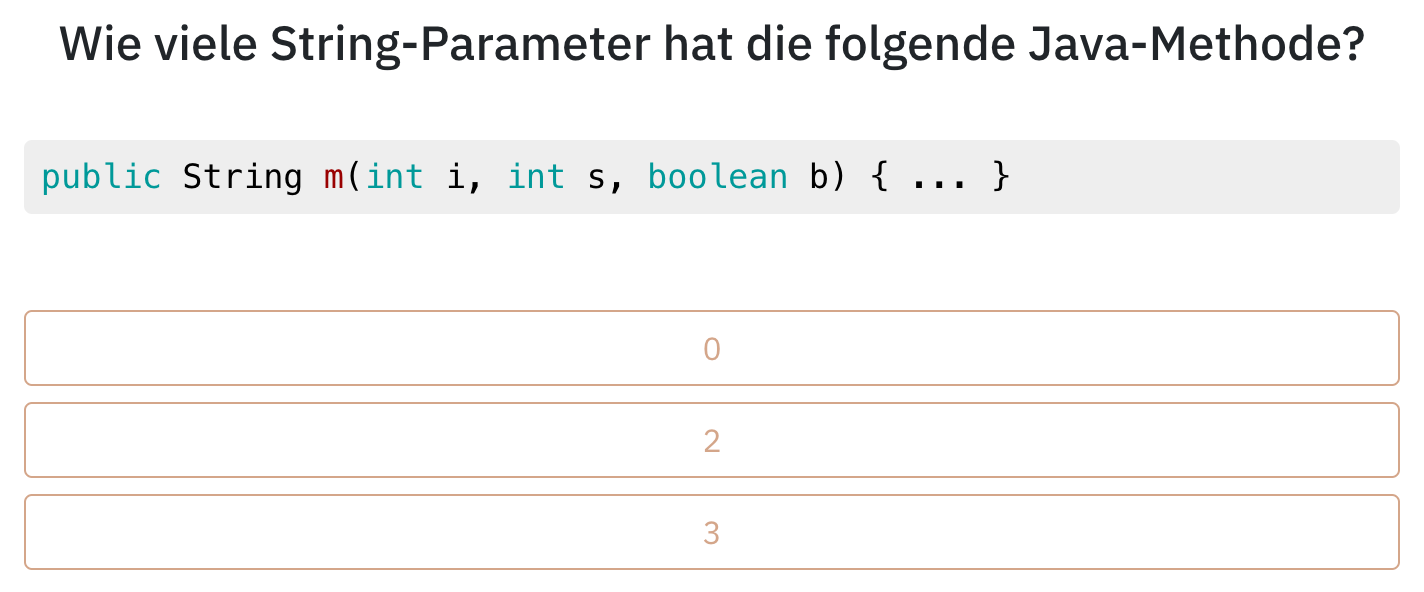
\includegraphics[width=\textwidth-1pt]{chapter/entwurf/bilder/weclare_fragment.png}}%
    \caption[Darstellung eines Code-Fragments in Weclare]{Darstellung eines Code-Fragments in Weclare (Quelltext als Code-Block ausgezeichnet)}
    \label{abb:weclare_code_fragment}
\end{figure}

Der zweite Kontext von Quelltexten in Fragestellungen ist das Einfügen von vollständigem, ausführbarem Code, in Form ganzer Java-Klassen. Solcher Code kann in Weclare direkt im Browser ausgeführt werden. So ein interaktives Code-Beispiel kann allerdings nur einmal pro Frage vorhanden sein und ist auch nicht Teil des Fließtexts. Eine entsprechende Editor-Komponente zum Einfügen solchen Codes sollte also auch funktional darauf zugeschnitten sein: Text-Formatierungen sind nicht mehr notwendig, stattdessen rücken Funktionen wie die korrekte Einrückung von Code-Zeilen und Zeilen-Nummerierungen in den Vordergrund.

Der Quill-Editor kann leider nicht in einem „Code only“-Modus betrieben werden, so dass eine zweite, unabhängige Editor-Komponente für interaktive Code-Abschnitte integriert wird. Mit CodeMirror\footnote{Offizielle Webseite: \url{https://codemirror.net/}} existiert eine sehr beliebte Bibliothek für diesen Zweck, die allerdings auch nicht explizit für den Einsatz im React-Framework bestimmt ist, so dass auch sie in Form einer Wrapper-Bibliothek namens \texttt{react-codemirror2}\footnote{Offizielle Webseite: \url{https://github.com/scniro/react-codemirror2}} zum Einsatz kommt.



\begin{figure}[H]
    \centering
    \setlength{\fboxsep}{0pt}
    \setlength{\fboxrule}{0.5pt}
    \fbox{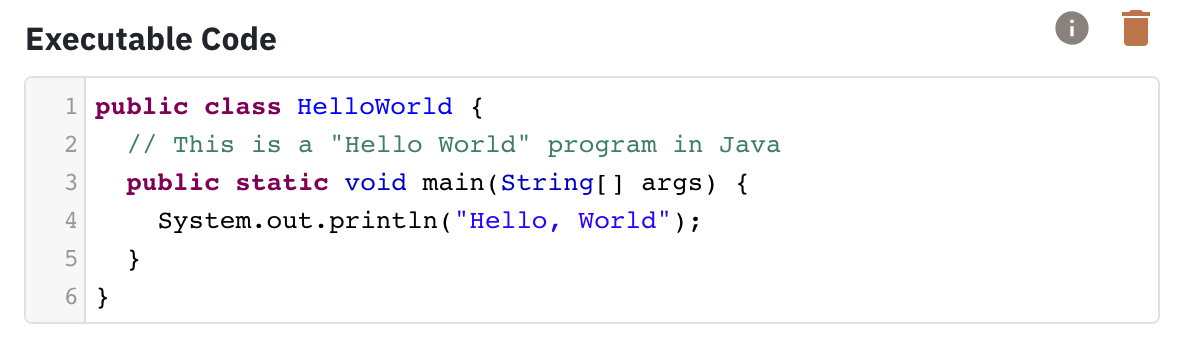
\includegraphics[width=\textwidth-1pt]{chapter/entwurf/bilder/weclare_codemirror.png}}
    \caption[Darstellung eines ausführbaren Java-Quelltexts in Weclare]{Darstellung eines ausführbaren Java-Quelltexts in Weclare mittels der CodeMirror-Bibliothek.}
    \label{abb:weclare_codemirror}
\end{figure}

\newpage
\section{Code-Ausführung im Browser via DoppioJVM}
\label{chap:ausfuehrung}
Normalerweise wird Java in einem zweistufigen Prozess ausgeführt. Zunächst wird eine plattformabhängige JVM geladen. Innerhalb dieser JVM wird der Java-Compiler (javac) aufgerufen. Dieser compiliert Java-Quelltext zu Java-Bytecode. Der Java-Bytecode kann dann von der JVM ausgeführt werden. Dieser Ablauf ist in der \ref{abb:java_execution} unter a) dargestellt.

Um Java in einem Browser auszuführen ergeben sich konzeptionell mindestens drei verschiedene Möglichkeiten, die in \ref{Abbildung 4.4} mit den Buchstaben b-d gekennzeichnet sind.

\begin{figure}[H]
    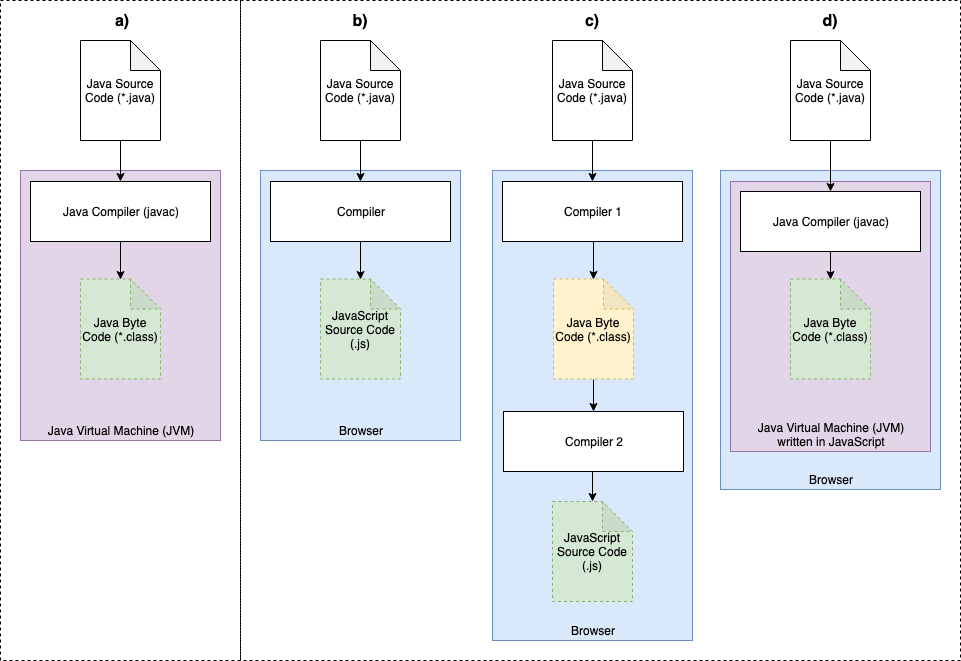
\includegraphics[width=14cm]{chapter/entwurf/bilder/Java_JavaScript_Execution.png}
    \centering
    \caption{Blubb}
    \label{abb:java_execution}
\end{figure}

\begin{itemize}
    \item \textbf{b:} Java-Quelltext wird mit einem Compiler direkt in JavaScript umgewandelt: Diese Variante ist konzeptionell sehr einfach. Zwar gibt es einige Programme, welche Java-Quelltext in JavaScript übersetzen können (zum Beispiel JSweet oder GWT), jedoch sind alle diese Programme entweder in Java selbst oder in anderen Programmiersprachen verfasst. Einen solchen Compiler, der selbst in JavaScript geschrieben wurde, gibt es bisher nicht. Es wäre möglich eines der besagten Programme auf einem separaten Server zu verwenden. Dies würde aber eine weitere Abhängigkeit von einem Server bedeuten, und damit der formulierten Kern-Anforderung widersprechen.
    \item \textbf{c:} Java-Quelltext wird mithilfe eines ersten Compilers in Java-Bytecode übersetzt. Anschließend wird der Java-Bytecode mit einem zweiten Compiler in JavaScript übersetzt. Auch hier ergibt sich das gleiche Problem wie in b). Zwar gibt es Programme, die den jeweiligen Teilschritt übernehmen könnten, jedoch ist keins davon in JavaScript verfasst, so dass es keine Lösung dafür im Browser gibt.
    \item \textbf{d:} Es wird eine JVM verwendet, die in JavaScript implementiert wurde. Mithilfe dieser JVM kann der javac-Compiler geladen werden, um Java-Quelltext in Java-Bytecode zu übersetzen und anschließend auszuführen. Eine solche JavaScript-JVM existiert bereits in Form eines Universitätsprojekt der University of Massachusetts unter dem Namen DoppioJVM. Der konzeptionelle Nachteil dieser Lösung liegt in der benötigten Datenmenge: Um eine komplette JVM im Browser auszuführen wird ebenfalls die Java Runtime Environment benötigt, deren Größe bei etwa 60 Megabyte liegt.
\end{itemize}

In Anbetracht der Tatsache, dass die Ausführung der Code-Beispiele im Browser exakt die gleichen Ergebnisse liefern soll, wie die Ausführung in einer lokalen JVM (zum Beispiel auch in Bezug auf Fehler beim Kompilieren), so ist die Variante d die bevorzugte Lösung und wurde im Rahmen dieser Arbeit in das entstandene CRS integriert.

DoppioJVM ist das Ergebnis der PLASMA-Forschungsgruppe der University of Massachusetts in Amherst, USA. Das Projekt wurde im Jahr 2014 im Rahmen einer wissenschaftlichen Arbeit veröffentlicht und wird von den Autoren selbst wie folgt beschrieben:

\begin{quotation}
„DoppioJVM is a robust prototype Java Virtual Machine (JVM) interpreter
that operates entirely in JavaScript. DoppioJVM implements all
201 bytecode instructions specified in the second edition of the
Java Virtual Machine Specification, supports multithreaded
programs, runs multiple languages that run on top of the JVM, and
implements many of the complex mechanisms and native functionality that JVM programs expect.“
\end{quotation}

Voraussetzung für den Betrieb von DoppioJVM ist ein weiteres Projekt der gleichen Forschungsgruppe: BrowserFS. Dabei handelt es sich um die Implementation eines NodeJS-kompatiblen Dateisystems innerhalb des Browsers. Somit können JavaScript-Programme, die eigentlich für die NodeJS-Laufzeitumgebung gestaltet sind (also Zugriffe auf ein Dateisystem ermöglichen) auch im Browser ausgeführt werden. BrowserFS emuliert ein Dateisystem auf Basis verschiedener Webstandards. So können für den Betrieb der DoppioJVM zum Beispiel die JRE-Komponenten über ein virtuelles Dateisystem bereitgestellt werden, welches auf dem asynchronen Nachladen basiert, oder andere Komponenten der JVM über den LocalStorage des Browsers.

Nachdem das BrowserFS-Dateisystem konfiguriert ist, kann DoppioJVM mit einer relativ einfachen Schnittstelle verwendet werden:

\begin{minipage}{\linewidth}
\begin{lstlisting}
new Doppio.VM.JVM(
  {
    doppioHomePath: "/sys",
    classpath: [".", "/sys/", "/tmp/"]
  },
  (err, jvmObject) => {
    jvmObject.runClass("Loader", [classname], exitCode => {
      if (exitCode !== 0) {
        console.log("JVM exited with an error");
      } else {
        console.log("JVM exited successfully");
      }
    });
  }
);
\end{lstlisting}
\end{minipage}

Die DoppioJVM muss bei jeder Verwendung neu instantiiert werden. Deswegen ist es erforderlich, dass die Kompilierung und Ausführung des gewünschten Java-Codes in einem Aufruf erfolgt. Dazu hat Java einige Möglichkeiten an Bord, die in Form der folgenden Loader-Klasse implementiert wurden:

\begin{minipage}{\linewidth}
\begin{lstlisting}
import javax.tools.*;
import java.lang.reflect.*;
import java.io.*;
import java.net.*;

public class Loader {
  public static void main(String[] args) {
    if (args.length == 0) {
      System.out.println("No class was found.");
      System.exit(1);
    }
    String className = args[0];
    String sourceFile = "/tmp/" + className + ".java";
    String classFile = "/tmp/" + className + ".class";

    System.out.println("Compiling found class '" + className + "'...");

    JavaCompiler compiler = ToolProvider.getSystemJavaCompiler();
    int result = compiler.run(null, null, null, sourceFile, "-d", "/tmp/");

    if (result == 0) {
      try {
        System.out.println("Compilation successful. Executing...");
        System.out.println("---");

        URLClassLoader classLoader = new URLClassLoader(
            new URL[] {new File(classFile).toURI().toURL()}, ClassLoader.getSystemClassLoader());
        Class<?> c = classLoader.loadClass(className);
        Method m = c.getDeclaredMethod("main", String[].class);
        m.invoke(null, new Object[] {});
        classLoader.close();

        System.out.println("Execution successfull");
      } catch (Exception e) {
        e.printStackTrace();
      }
    } else {
      System.out.println("Could not compile");
    }
  }
}
\end{lstlisting}
\end{minipage}

\begin{figure}[H]
    \centering
    \setlength{\fboxsep}{0pt}
    \setlength{\fboxrule}{0.5pt}
    \fbox{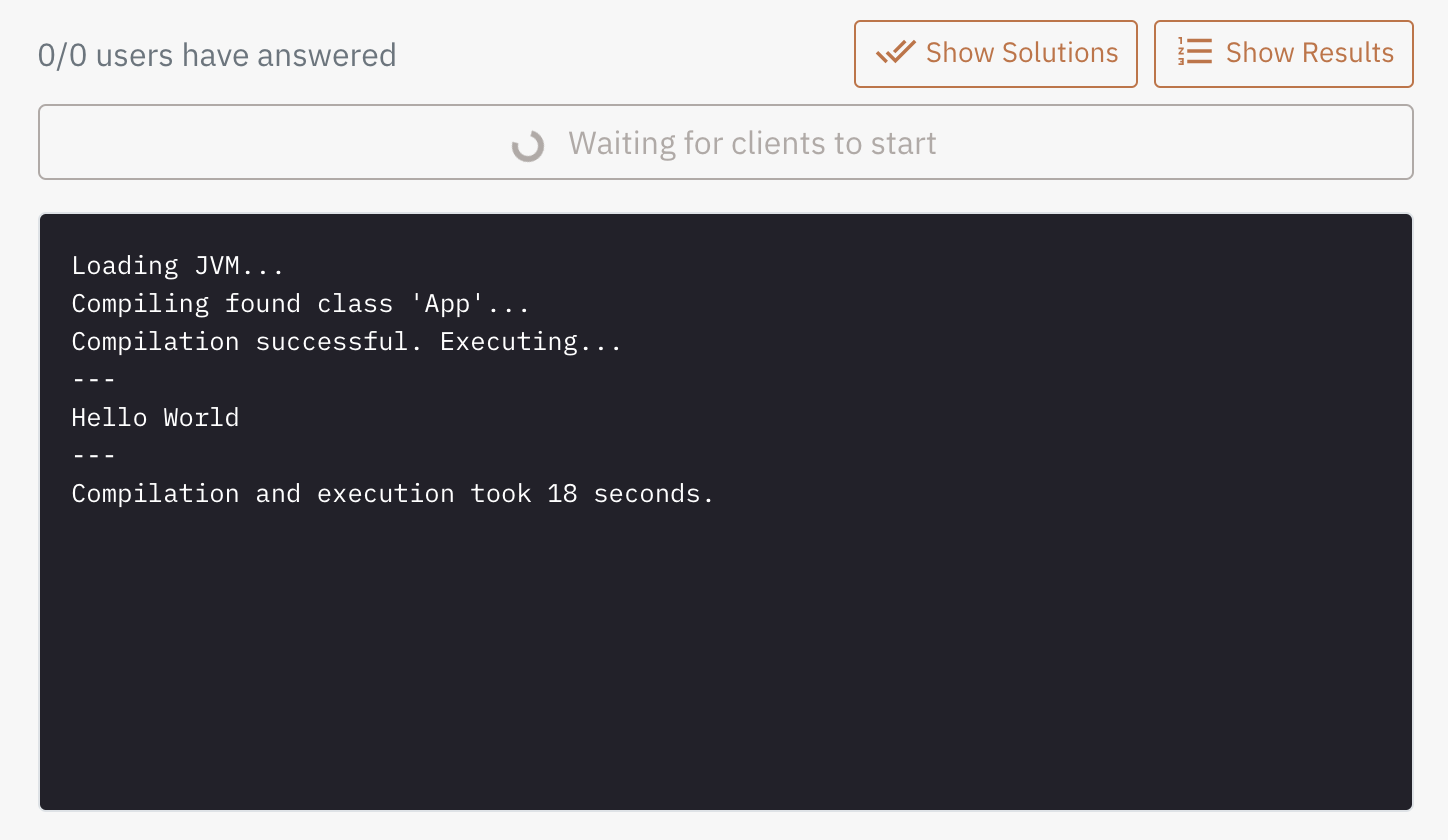
\includegraphics[width=\textwidth-1pt]{chapter/entwurf/bilder/weclare_jvm_console.png}}
    \caption{Ausführung einer Java-Klasse in Weclare mittels DoppioJVM.}
    \label{abb:weclare_jvm_console}
\end{figure}

